\documentclass[journal]{vgtc}                % final (journal style)
%\documentclass[review,journal]{vgtc}         % review (journal style)
%\documentclass[widereview]{vgtc}             % wide-spaced review
%\documentclass[preprint,journal]{vgtc}       % preprint (journal style)

%% Uncomment one of the lines above depending on where your paper is
%% in the conference process. ``review'' and ``widereview'' are for review
%% submission, ``preprint'' is for pre-publication, and the final version
%% doesn't use a specific qualifier.

%% Please use one of the ``review'' options in combination with the
%% assigned online id (see below) ONLY if your paper uses a double blind
%% review process. Some conferences, like IEEE Vis and InfoVis, have NOT
%% in the past.

%% Please use the ``preprint''  option when producing a preprint version
%% for sharing your article on an open access repository

%% Please note that the use of figures other than the optional teaser is not permitted on the first page
%% of the journal version.  Figures should begin on the second page and be
%% in CMYK or Grey scale format, otherwise, colour shifting may occur
%% during the printing process.  Papers submitted with figures other than the optional teaser on the
%% first page will be refused. Also, the teaser figure should only have the
%% width of the abstract as the template enforces it.

%% These few lines make a distinction between latex and pdflatex calls and they
%% bring in essential packages for graphics and font handling.
%% Note that due to the \DeclareGraphicsExtensions{} call it is no longer necessary
%% to provide the the path and extension of a graphics file:
%% 
\includegraphics{diamondrule} is completely sufficient.
%%
\ifpdf%                                % if we use pdflatex
  \pdfoutput=1\relax                   % create PDFs from pdfLaTeX
  \pdfcompresslevel=9                  % PDF Compression
  \pdfoptionpdfminorversion=7          % create PDF 1.7
  \ExecuteOptions{pdftex}
  \usepackage{graphicx}                % allow us to embed graphics files
  \DeclareGraphicsExtensions{.pdf,.png,.jpg,.jpeg} % for pdflatex we expect .pdf, .png, or .jpg files
\else%                                 % else we use pure latex
  \ExecuteOptions{dvips}
  \usepackage{graphicx}                % allow us to embed graphics files
  \DeclareGraphicsExtensions{.eps}     % for pure latex we expect eps files
\fi%

%% it is recomended to use ``\autoref{sec:bla}'' instead of ``Fig.~\ref{sec:bla}''
\graphicspath{{figures/}{pictures/}{images/}{./}} % where to search for the images

\usepackage{microtype}                 % use micro-typography (slightly more compact, better to read)
\PassOptionsToPackage{warn}{textcomp}  % to address font issues with \textrightarrow
\usepackage{textcomp}                  % use better special symbols
\usepackage{mathptmx}                  % use matching math font
\usepackage{times}                     % we use Times as the main font
\renewcommand*\ttdefault{txtt}         % a nicer typewriter font
\usepackage{cite}                      % needed to automatically sort the references
\usepackage{tabu}                      % only used for the table example
\usepackage{booktabs}                  % only used for the table example
%% We encourage the use of mathptmx for consistent usage of times font
%% throughout the proceedings. However, if you encounter conflicts
%% with other math-related packages, you may want to disable it.

%% In preprint mode you may define your own headline. If not, the default IEEE copyright message will appear in preprint mode.
%\preprinttext{To appear in IEEE Transactions on Visualization and Computer Graphics.}

%% In preprint mode, this adds a link to the version of the paper on IEEEXplore
%% Uncomment this line when you produce a preprint version of the article 
%% after the article receives a DOI for the paper from IEEE
%\ieeedoi{xx.xxxx/TVCG.201x.xxxxxxx}

%% If you are submitting a paper to a conference for review with a double
%% blind reviewing process, please replace the value ``0'' below with your
%% OnlineID. Otherwise, you may safely leave it at ``0''.
\onlineid{0}

%% declare the category of your paper, only shown in review mode
\vgtccategory{Research}
%% please declare the paper type of your paper to help reviewers, only shown in review mode
%% choices:
%% * algorithm/technique
%% * application/design study
%% * evaluation
%% * system
%% * theory/model
\vgtcpapertype{please specify}

%% Paper title.
\title{Towards Trustworthy Transformer Models in Machine Learning}

%% This is how authors are specified in the journal style

%% indicate IEEE Member or Student Member in form indicated below
\author{Ahmad Rashid, Siqing Huo, Temiloluwa P. Femi-Gege and Shaikh S. A. Shimon}
\authorfooter{
%% insert punctuation at end of each item
\item
 Ahmad Rashid is with University of Waterloo and Vector Institute. E-mail: a9rashid@uwaterloo.ca.
\item
 Siqing Huo is with University of Waterloo. E-mail: s2huo@uwaterloo.ca
\item
 Temiloluwa P. Femi-Gege is with University of Waterloo. E-mail: tpfemige@uwaterloo.ca
\item
 Shaikh S. A. Shimon is with University of Waterloo. E-mail: ssarefin@uwaterloo.ca
}

%other entries to be set up for journal
\shortauthortitle{Biv \MakeLowercase{\textit{et al.}}: Global Illumination for Fun and Profit}
%\shortauthortitle{Firstauthor \MakeLowercase{\textit{et al.}}: Paper Title}

%% Abstract section.
\abstract{
Trustworthiness in Machine Learning (ML) is one of the most important factor for domain experts with low ML expertise to deploy ML solutions in critical environments such as Healthcare and Control Systems. Our work focuses on increasing reliability and understanding of state-of-the art (SOTA) Natural language Processing (NLP) models in order to deploy them to aforementioned critical environments for general domain experts with low ML expertise. Studies have shown that transformers models (current SOTA for NLP) are vulnerable to adversarial attacks. Existing visualization techniques for transformer models do not support side-by-side model or text sequence comparison to compare model behavior changes under adversarial attack. In this work, we present visualization tool which can help compare attention patterns of different transformer models, compare between original and adversarial examples and provide a mechnism for filtering attention heads. Our aim is to increase transformer model interpretability for domain experts and help them understand how the model behavior changes with slight perturbations of data and also help ML experts to take appropriate measures while training to reduce this vulnerability. 
%Machine Learning (ML) has made substantial progress over the last decade with the help of a strong deep learning toolkit, larger data sets, better optimization algorithms, faster and cheaper computation and an open, vibrant and diverse research community. It has inspired many new technologies such as self-driving cars, personalized healthcare, drug discovery, personalized advertising, machine translation, etc. This has prompted questions into the reliability and the trustworthiness of the algorithms since mistakes can gravely affect many people. Under ML trustworthiness, researchers are exploring diverse areas such as robustness and generalization, privacy, data deletion, fairness and interpretability. In this work we will explore natural language processing and visualize the internal representations of state-of-the-art transformer networks when exposed to adversarial examples. We will use and develop existing visualization to diagnose model vulnerabilities and suggest improvements which can lead to robust Transformer Models in ML.   
} % end of abstract

%% Keywords that describe your work. Will show as 'Index Terms' in journal
%% please capitalize first letter and insert punctuation after last keyword
\keywords{Machine Learning, Transformers, Visualization, Robustness, Reliability}

%% ACM Computing Classification System (CCS). 
%% See <http://www.acm.org/class/1998/> for details.
%% The ``\CCScat'' command takes four arguments.

\CCScatlist{ % not used in journal version
 \CCScat{K.6.1}{Management of Computing and Information Systems}%
{Project and People Management}{Life Cycle};
 \CCScat{K.7.m}{The Computing Profession}{Miscellaneous}{Ethics}
}

%% A teaser figure can be included as follows
% \teaser{
%   \centering
%   
\includegraphics[width=\linewidth]{CypressView}
%   \caption{In the Clouds: Vancouver from Cypress Mountain. Note that the teaser may not be wider than the abstract block.}
%   \label{fig:teaser}
% }

%% Uncomment below to disable the manuscript note
%\renewcommand{\manuscriptnotetxt}{}

%% Copyright space is enabled by default as required by guidelines.
%% It is disabled by the 'review' option or via the following command:
% \nocopyrightspace


\vgtcinsertpkg

%%%%%%%%%%%%%%%%%%%%%%%%%%%%%%%%%%%%%%%%%%%%%%%%%%%%%%%%%%%%%%%%
%%%%%%%%%%%%%%%%%%%%%% START OF THE PAPER %%%%%%%%%%%%%%%%%%%%%%
%%%%%%%%%%%%%%%%%%%%%%%%%%%%%%%%%%%%%%%%%%%%%%%%%%%%%%%%%%%%%%%%%

\begin{document}

%% The ``\maketitle'' command must be the first command after the
%% ``\begin{document}'' command. It prepares and prints the title block.

%% the only exception to this rule is the \firstsection command
\firstsection{Introduction}

\maketitle

Recent advances in Machine Learning (ML) have inspired new applications and technologies such as medicine, advertising, drug discovery, self-driving and more. Machine learning platforms have seen an increased deployment to critical application sectors such as control systems or healthcare to create predictive models trained with ground truth data. The end-users of such ML platforms have domain expertise in the respective application sectors, but do not have expertise in ML domain and treat ML platform as black-boxes.Deploying ML platforms in these critical application sectors require a high-degree of testing and verification. However, recent studies have shown that lay-users trust on such black box prediction models depend on understanding the inner working of the ML model\cite{DoshiVelez2017Towards} \cite{DBLP:journals/corr/Lipton16a} \cite{DBLP:journals/corr/RibeiroSG16}, not just the reported accuracy score of said black-box models. Trustworthy ML studies data privacy, data deletion, algorithm robustness, algorithm fairness and interpretability among other disciplines. Our work will focus on robustness and interpretability of  natural language processing (NLP) predictive models.



%   Our work focuses on evaluating the vulnerability of to adversarial examples and using visualizations to enhance the interpretability. 

\begin{figure*}[tb]
    \centering
    
    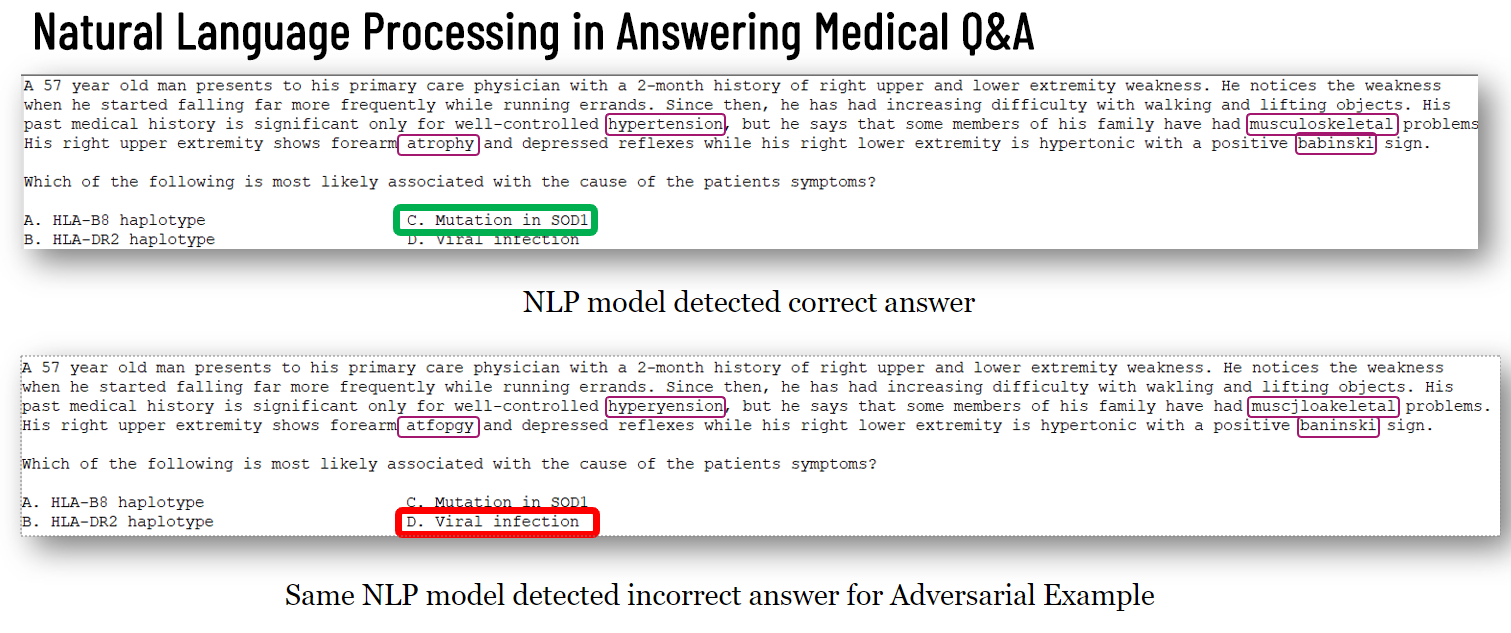
\includegraphics[width=16cm]{figures/adversarialExample.jpg}
    \caption{Demonstrating the effect of adversarial examples on NLP classifier predicting the cause of a patient's symptoms }
    % We show anframework in-domain sample, a sample from the HANS evaluation set and one produced by our universal adversarial 
    \label{fig:adversarialExample}
    
\end{figure*}


Currently, NLP systems are mostly built using Deep Neural Networks (DNNs), which,  have achieved state-of-the-art (SOTA) results on diverse applications such as machine translation, speech recognition, natural language understanding, summarization etc. However, it has been observed across various disciplines of ML that DNN classifiers are vulnerable to adversarial examples - small,  label preserving perturbations of data.  In machine translation, it was shown that replacing a word by its synonym can sometimes lead to a nonsensical translation in commercial systems~\cite{cheng2019robust}. Another study demonstrated that adding a small amount of character level noise or natural noise~\cite{belinkov2018synthetic} can significantly reduce the performance SOTA translation systems. In natural language inference (NLI), \cite{mccoy2019right} demonstrated that statistical models learnt syntactical heuristics that are data set specific and not general. The common theme between all these works is that they demonstrate that DNNs tend to learn surface level patterns or `shortcuts'~\cite{geirhos2020shortcut} in the data. Figure~\ref{fig:adversarialExample} shows the effect of changing a few characters in a paragraph can change the prediction of an NLP classifier in the medical domain.

In this work, we focus on the interpretability and robustness of the Transformer model~\cite{vaswani2017attention}, a SOTA DNN model in NLP, when evaluated on adversarial examples. Transformer models process the entire input data at once and derive context between text tokens through a mechanism called attention. The capability of processing the entire input data at once compared to other models processing one token at a time allows Transformer models to be massively parallelizable. 

Whereas recent works have explored the effect of adversarial examples on transformers~\cite{jin2019bert}, most of the works only measure the effect on summary statistics such as accuracy and F1 score. They have no way of identifying the cause of the vulnerability and are unable to prescribe any solution. In this work, we aim to focus on improving transformer visualizations to visualize model layers under the influence of adversarial examples. We focus on visualization of attention layers to identify patterns which can help ML practitioners, non-technical domain experts and linguists understand how the transformer NLP model behavior changes with respect to adversarial attacks, and help them guide ML practitioners to improve the NLP model in question. We achieve this by providing side-by-side visual comparison of the attention layers between a text sequence and it's adversarial example pair for a Transformer model. Moreover, we also provide side-by-side comparison of two different models and come up with mechanisms which help guide the user which attention module to look at among multiple attention layers. To the best of our knowledge, existing visualization solutions for transformer models do not provide such a visual comparison toolkit for comparing models or side-by-side sequence comparisons for attention based models. Our work can help users identify the reasons for vulnerability to adversarial attacks and provide feedback on how to train ML models to be more robust.

%Recent advances in Machine Learning (ML) are in part due to deep neural networks (DNNs), which are powerful function approximators. DNNs have achieved ground-breaking results on the protein folding problem~\cite{jumper2021highly}, have reportedly reached human-level performance on object recognition~\cite{he2015delving}, form the backbone of commercial machine translation systems~\cite{45610} and have beaten world-class human Go and poker players among other impressive achievements~\cite{silver2016mastering,moravvcik2017deepstack}. Even during the COVID-19 pandemic, deep learning algorithms were at the forefront of ML solutions for detecting and predicting the outcome of COVID in patients. In a systemic review of 2,212 studies~\cite{roberts2021common}, reduced to 62 after various stages of screening, it was reported that more than half the works used DNNs. Unfortunately, none of the models identified were of potential clinical use. One of the main concerns was that, more than 80\% of the DNN studies conducted no sensitivity analysis or robustness test of their model, and about 60\% did not sufficiently report issues around generalization.

%It has been observed across various disciplines of ML that DNN classifiers are vulnerable to even small perturbations of data. In computer vision (CV), researchers proposed adversarial examples~\cite{szegedy2013intriguing}, i.e., small, intentional image perturbations, which are indiscernible to humans, but can cause the classifier to make a mistake. In machine translation, it was shown that replacing a word by its synonym can sometimes lead to a nonsensical translation in commercial systems~\cite{cheng2019robust}. Another study demonstrated that adding a small amount of character level noise or natural noise~\cite{belinkov2018synthetic} can significantly reduce the performance of state-of-the-art (SOTA) translation systems. In natural language inference (NLI), \cite{mccoy2019right} demonstrated that statistical models learnt syntactical heuristics that are data set specific and not general. The common theme between all these works is that they demonstrate that DNNs tend to learn surface level patterns or `shortcuts'~\cite{geirhos2020shortcut} in the data.

%In this work, we focus on the reliability and robustness of a state-of-the-art (SOTA) model of DNN called Transformer Networks. Transformer networks process the entire input data at once and derive context between text tokens through a mechanism called attention. The capability of processing the entire input data at once compared to other models processing one token at a time allows transformer models to be massively parallelized. These transformer networks are currently SOTA no diverse NLP applications such as machine translation, speech recognition, natural language understanding etc. displacing recurrent neural networks (RNNs) and convolutional neural networks (CNNs). 

%Whereas recent works have explored the effect of adversarial examples on transformers~\cite{jin2019bert}, most of the works only measure the effect on summary statistics such as accuracy and F1 score. They have no way of identifying the cause of the vulnerability and are unable to prescribe any solution. In this work, we aim to focus on improving transformer visualizations to visualize model layers under the influence of adversarial examples. We will focus on both on both summary statistics and visualization of attention layers to identify patterns which can help us diagnose training vulnerabilities and provide actionable insights.

% Recent works by Mahmood \MakeLowercase{\textit{et al.}}~\cite{https://doi.org/10.48550/arxiv.2104.02610} show that although CNN models have been carefully studied with respect to adversarial problems, transformer models against adversarial examples is yet to be explored in detail. Most of the work done adversarial problems exploration in transformer models employ traditional performance measurement techniques to benchmark transformer models against adversarial attacks. 


\section{Related Works}

\subsection{Pre-trained Language Models}
Attention is a mechanism to measure how different elements in two sequences are related to each other in terms of an attention or affinity score. Although attention was proposed in NLP to improve the memorization of long sequence by recurrent neural networks, Vaswani \MakeLowercase{\textit{et al.}}~\cite{vaswani2017attention} proposed a self-attention based architecture called the transformer and demonstrated that it was state-of-the-art (SOTA) on machine translation. Devlin \MakeLowercase{\textit{et al.}}~\cite{devlin2019bert} applied transformers to language modeling (LM) and proposed Bidirectional Encoder Representation from Transformers (BERT), a masked language modeling (MLM) based architecture trained on 16 GBs of data. Traditional LMs are left to right and autoregressive whereas MLMs randomly mask a few tokens of the input sequence and train to predict them. BERT demonstrated that MLMs learn a better language representation and can be fine-tuned on different tasks, such as question answering, natural language inference, sentiment analysis etc. and achieve SOTA performance. This pre-train (LM on a large corpus) then fine-tune (on the target data and application) is now the dominant paradigm in NLP and the underlying models are referred to as pre-trained language models (PLMs). Current PLMs are composed of hundreds of billions of parameters and are trained on terabytes of data.  

\subsection{Adversarial Examples}
In machine learning - \textit{adversarial examples} are small data perturbations which are indiscernible to humans but can confuse a neural network classifier. This concept was first identified in computer vision~\cite{Goodfellow2015ExplainingAH,DBLP:journals/corr/KurakinGB16,labacacastro2021universal}. The traditional approach to counter adversarial example based attacks is to add gradient-based perturbation on continuous input spaces~\cite{Goodfellow2015ExplainingAH,DBLP:journals/corr/KurakinGB16}. 

Adversarial examples have recently been extended into domains outside of computer vision as well, and NLP is one of such domain.  Jin \MakeLowercase{\textit{et al.}} proposed \textit{TextFooler}~\cite{jin2019bert} tool to measure robustness of NLP models against adversarial text attacks. This tool is capable of generating adversarial text examples, as well as replacing the most semantically important words based on model output. Others~\cite{zhu2020freelb,ghaddar2021context,ghaddar-etal-2021-end,rashid-etal-2021-mate} have looked into introducing adversarial examples as data augmentation in the training phase of NLP models to improve generalization and robustness. Text - unlike images is discrete, and perturbing the gradient of word embeddings can lead to nonsensical changes. Ribiero \MakeLowercase{\textit{et al.}} explored rule-based methods to generate semantically meaningful adversarial text examples for probing NLP model robustness.  Hybrid models (models based but condition on rules) such as Textfooler are most commonly used. 

% In natural language inference (NLI)~\cite{mccoy2019right} identified a few heuristics patterns in the MNLI~\cite{williams-etal-2018-broad} dataset and designed adversarial examples for that. Similarly \cite{zhang2019paws} does the same for the task of paraphrase detection on the QQP~\cite{wang2017bilateral} dataset. Although these works test for only a few selected patterns, the adversarial datasets are of high quality and have been widely demonstrated to confuse SOTA classifiers. 

Several visualization techniques have been developed to allow users to investigate the robustness of ML models against adversarial examples. DetectorDetective ~\cite{DetectorDetective} visualizes feature maps extracted by the selected module for benign and adversarial images side-by-side. Our design also shows side-by-side comparisons of models' internals in response to benign and adversarial inputs. \textit{Bluff}~\cite{Bluff} is another tool that compares activation pathway traversal for both benign and adversarial inputs. Bluff also aims to help users understand the roles of neurons in complex deep neural models which lack semantic meanings. When hovering over a neuron in \textit{Bluff}, dataset examples (which activate the neuron highly) are shown, as well as the feature visualization for the corresponding neuron. Our work will also provide users more context through interactions to help them understand the complex internals of the models.

Visualizations of adversarial examples have been mainly studied in the context of images, general deep neural networks, and neuron activations. Our work will built on these visual, side-by-side comparisons of model's behavior with respect to benign and adversarial examples, and tailor the solution toward text and the Transformer model.


\subsection{NLP Visualization}
On the other hand, existing visualizations for NLP are not tailored for investigating the robustness of the models against adversarial examples. However, these general purpose visualization techniques do provide useful insights.  ACTIVIS ~\cite{ACTIVIS} enables subset-level visualization and allows users to customize subsets by applying any function to any combination of features. Texts are not as structured as tabular data, thus the functionality of customizing function to generate subset can be very helpful in producing useful subsets. We aim to support subset-level visualization and give user more freedom in defining subsets.
SEQ2SEQ-VIS ~\cite{SEQ2SEQVIS} facilitates debugging sequence-to-sequence models. It offers the ability to explore neighborhood of encoder states and decoder states, to visualize attention and probability scores of likely next words, and to visualize the top K considered options at each prediction step as a beam search tree. Users can explore the model's behavior by changing words at each step, or altering the assigned attention values. These interactions are very useful for probing the model's behavior and can be extended to exploring how an adversarial example can succeed.

\subsection{Transformer Visualization}
Following the success of BERT and subsequent PLMs, a number of works have focussed exclusively on visualizing transformer based PLMs. BertViz~\cite{vig-2019-multiscale} builds on existing visualizations, such as matrix heatmaps, to view attention. It is capable of helping visualize models such as GPT-2~\cite{radford2019language} which is a decoder-only model and BERT which is an encoder-only model. Bertviz has three views - \textit{Attention-head view}, \textit{Model view} and \textit{Neuron view} incorporated in the visualization system. They attempt to visualize the computation of vectors using colour to show magnitude of dot products. The tool adds interactions that allow users to visualize the computed attention at various layers. However the visualization creates a  lot of cognitive load when figuring out what the color and magnitude in each position of the vectors means. Also, the Bertviz tool can not load other transformer models - hence not supporting side-by-side transformer model comparisons. Also, it does not support side by side comparison of attention heads for multiple examples (for example - a text sequence and it's paired adversarial text sequence). 

% Bertviz has three views - \textit{Attention-head view}, \textit{Model view} and \textit{Neuron view} incorporated in the visualization system. Attention patterns produced by individual attention heads can be viewd in the Attention-head view, providing an alternate way to visualize the heat map matrix representation of attention heads. The \textit{attention head} view also provides the added benefit of supporting interactivity. Some of the supported interactions allow users to choose the specific layer for the attention head users want to visualize. One use case of being able to visualize attention heads is to detect model bias. The \textit{model view} provides a high-level view of the attention across all the models layers. This can identify recurring patterns that may help debug cases where the model performs poorly. The \textit{neuron view} visualizes explanations as to how attention is computed. They attempt to visualize the computation of vectors using colour to show magnitude of dot products. The tool adds interactions that allow users to visualize the computed attention at various layers.



Aken \MakeLowercase{\textit{et al.}} proposed VisBERT~\cite{aken2020visbert} tool designed to visualize internal state of BERT model for Question-Answering tasks. It visually identifies distinct phases in BERT transformation to offer insights about failed predictions. However, VisBERT does not provide any visual information on attention heads in different layers, and different transformer models can not be compared side by side. Also, similar to Bertviz - it lacks the capability of supporting side by side comparison of multiple text sequences. 

Hoover \MakeLowercase{\textit{et al.}} developed ExBERT~\cite{hoover-etal-2020-exbert} - a transformer model and corpus agnostic visualization tool to provide insights to contextual representation meaning by aggregating annotations of matching similar contexts. Although ExBERT tool is transformer model agnostic - like VisBERT and Bertvis it lacks the capability of comparing multiple transformer models , or multiple text sequences side by side. Also - the tool has no way of loading other fine-tuned transformer models except for preloaded BERT and GPT-2. 

AttViz~\cite{skrlj-etal-2021-exploring} online toolkit offers visual inspection of distribution of attention values across token sequence. It also supports integrating existing transformer libraries in PyTorch. Similar to previously mentioned transformer visualization tools - it also lacks the capability to compare multiple models or text sequences side-by-side. Also, the underlying infrastructure is tightly coupled with BERT-base transformer model, and other transformer models can not be swapped in. 

% Yann Lecunn \MakeLowercase{\textit{et al.}} developed TransformerVis~\cite{DBLP:journals/corr/abs-2103-15949} which utilized dictionary learning to provide detailed visualization of transformers and show hierarchical semantic representation for each stage. Dunn \MakeLowercase{\textit{et al.}}~\cite{9582700} developed a context-sensitive visualization method for BERT based transformer model highlighting most influential words from a token sequence contributing to its classification. These holistic visualization techniques typically integrate most transformer components and provide detailed summaries. However, like previously mentioned visualization tools - they also lack the capability to compare transformer models side by side, or compare multiple text sequences in same model side by side to notice differences in attention heads. 

Our work focuses on addressing this gap of comparing multiple BERT-based transformer models side by side, as well as comparing a text sequence and it's paired adversarial sequence against the same transformer model to visualize the changes in the attention head and neuron activity. We also incorporated the finding in ~\cite{clark2019does} that attention heads attend to specific syntactic information of the input sentence to provide users more context. This visualization will help domain experts better understand NLP model behavior in the presence of adversarial examples. Although our solution is focused on NLP transformer model - it works well to support any NLP ML model with attention mechanism. 

\section{Methodology}

To demonstrate our visualization on a concrete NLP task, we chose the important language understanding problem of NLI. In this problem typically we are given a pair of sentences, the first is the premise and the second is the hypothesis. The problem is to classify whether premise entails the hypothesis, contradicts it or is neutral. These problems are important for chatbots and dialogue systems.

\subsection{Model and Dataset}

Our base transformer is BERT which is a pre-trained language model based on the transformer architecture. We will take the BERT-base model (12 layers, 12 attention heads) from Google's official github repository~\footnote{https://github.com/google-research/bert/.}. 

The dataset we evaluate on is the MNLI dataset~\cite{williams-etal-2018-broad} a widely reported on, crowd-sourced, multi-domain NLI dataset. Figure~\ref{fig:textfooler} gives shoes an adversarial example where changing a single word (occupation) to its synonym (job) can lead to a change in prediction by a machine learning model.

\begin{figure}[tb]
    \centering
    
    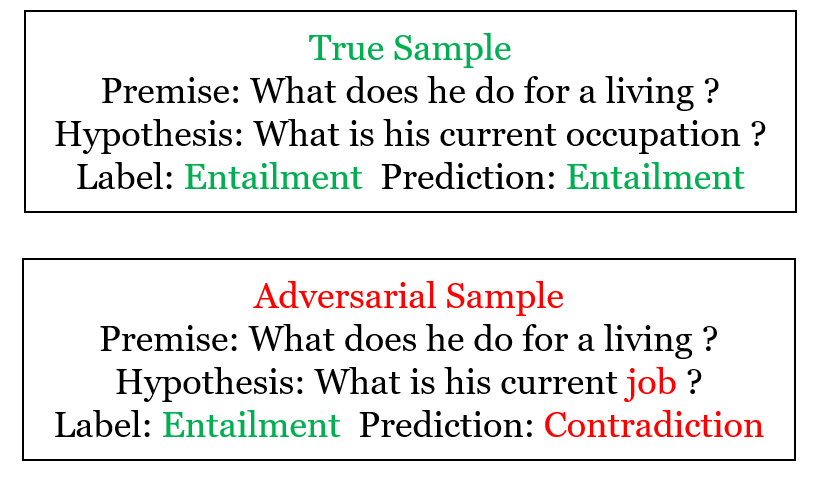
\includegraphics[width=8cm]{figures/textfooler2.png}
    \caption{Highlighting the differences between in domain and adversarial samples. The model makes an error on the TextFooler samples.}
    % We show anframework in-domain sample, a sample from the HANS evaluation set and one produced by our universal adversarial 
    \label{fig:textfooler}
    
\end{figure}

We fine-tune a pre-trained BERT model on the MNLI dataset and then evaluate it on the given evaluation (or benign) set and the adversarial set. The adversarial examples are generated by a model based system called Textfooler~\cite{jin2019bert}. The authors have shared 1000 samples that they generated for the MNLI dataset for BERT. We used the provided adversarial samples instead of generating them ourselves. As an additional step we manually verified the quality of the adversarial examples and then filtered out the ones which changed the label, semantics or were grammatically incorrect. 

%  We also use a second adversarial dataset called HANS~\cite{mccoy2019right} which is generated based on rules and exploits the artifacts present in the MNLI dataset. As an example the authors observe that whenever there is a significant overlap between the premise and the hypothesis in MNLI the correct label is usually an entailment. So they design examples where there is an overlap but the relationship can be a contradiction or neutral. 

% The literature suggests that larger (more parameters and training data) pre-trained models are more robust to adversarial evaluation~\cite{li2021select} and fine-tuning although neccessary for a target task makes the model more brittle. We will use visualization to compare models of different sizes and ones which are fine-tuned versus those which are not fine-tuned.

\subsection{Pipeline}


\begin{figure}
    \centering
    
    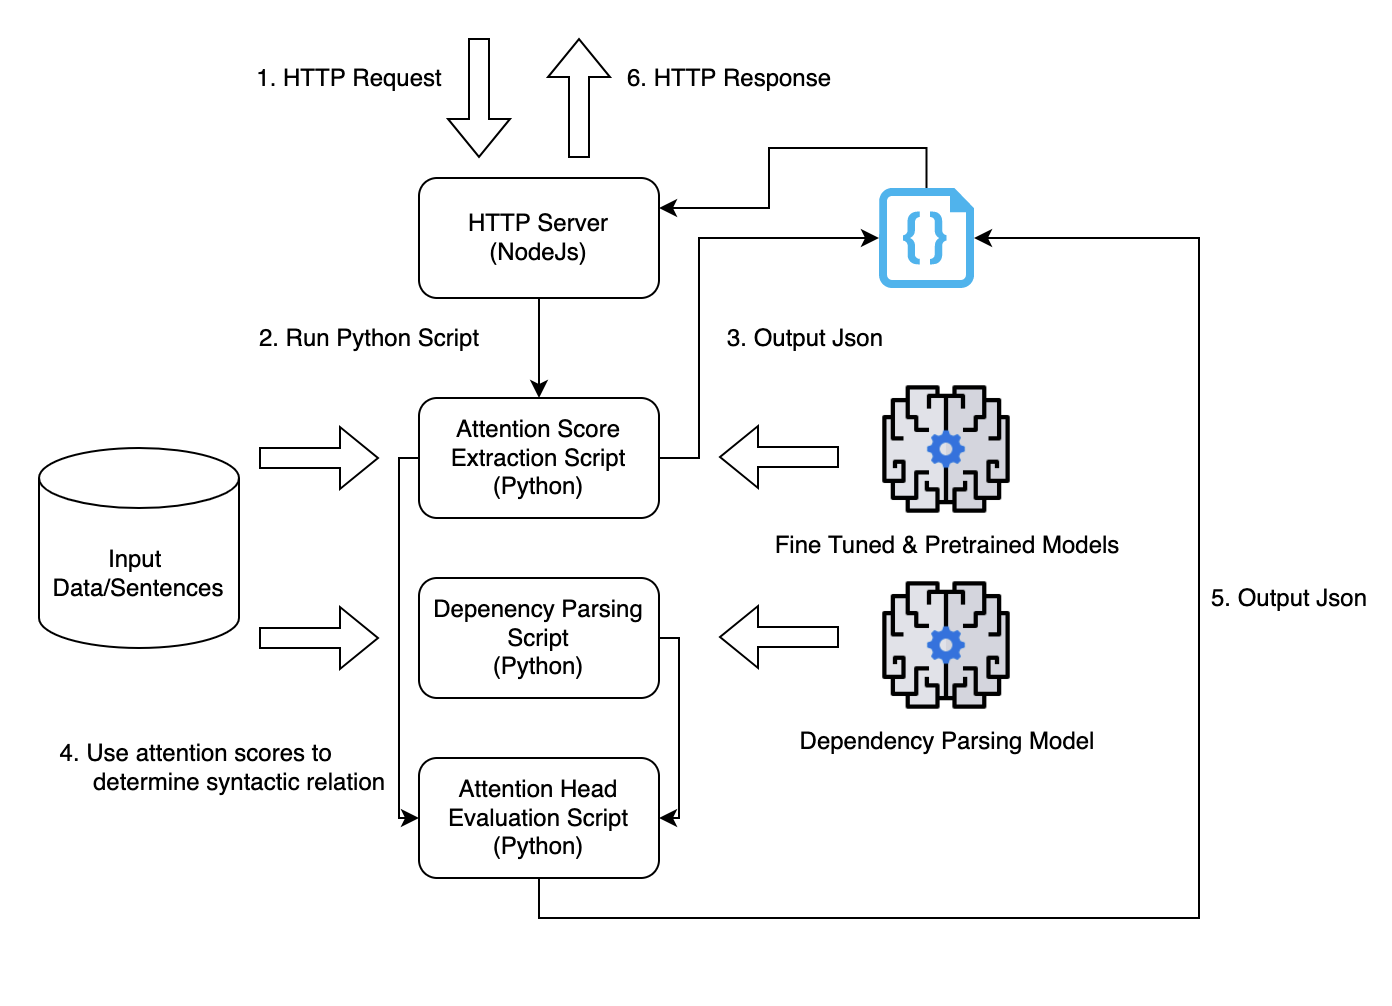
\includegraphics[width=8cm]{figures/pipeline.png}
    \caption{Overview of the Pipeline}
    \label{fig:pipeline}
    
\end{figure}

We present the overall architecture in the pipeline diagram in Figure~\ref{fig:pipeline}. Building on the work done in \cite{clark2019does} we extract the attention head scores for each model and instance which will be chosen by users. The BERT-base model, which we experimented on, has 12 layers and 12 attention heads which leads to 144 different attention heads. This can lead to a visual overload and no guidance as to where to start looking at in order to make sense of the prediction. Prior work~\cite{clark2019does} has demonstrated BERT has some understanding of syntactical relations of words. 

\begin{figure}[h]
    \centering
    
    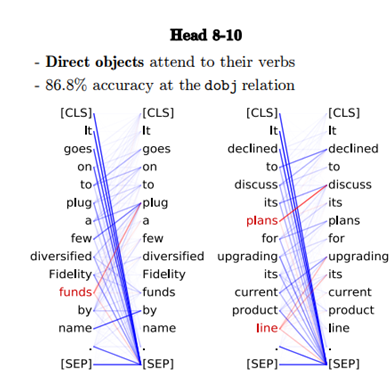
\includegraphics[width=8cm]{figures/syntax.png}
    \caption{Syntax relationship learnt by Attention head.}
    \label{fig:syntax}
    
\end{figure}

Figure~\ref{fig:syntax} shows that layer 8 attention head 10 for a pre-trained model learns direct object relationships with an 86.6\% accuracy. One of the main novelty of our work is that we classify which syntax information each attention head learns and use this information to select which attention head to analyze.The extracted scores for each attention head are passed into a classifier which outputs the syntactic relation which the attention head has learned. 

To generate the data which we provide to our visualization, we developed a backend that consists of various scripts that are executed for a baseline pre-trained model and a fine-tuned model. Our datasets were also separated into 2 groups, adversarial examples and benign examples. We first used a script to extract the self attention scores for a given input sequence from each list. The output of this script is an object array containing the original sentence, tokenized version of the sentence, a flag indicating whether it is adversarial or benign, a pair id which facilitates associating the sentence with its corresponding adversarial/benign sample, and a self attention scores matrix. In order to generate information about the syntactic relation a head focuses on, we pass our input sentences into a dependency parser ~\cite{lalparser} which identifies the true syntactic relations for each pair of tokens. The syntactic relation labels are compared with the attention scores for an attention head and serve as the true labels that help evaluate what syntactic relation a head focuses on. The outputs from both scripts are served to the frontend to be plotted for users. Our backend is built on NodeJs while the frontend is a React application.


\subsection{Visualization and Interaction}
Most existing transformer visualizations~\cite{vig-2019-multiscale, aken2020visbert, vskrlj2020attviz, kobayashi-etal-2020-attention} show only a single instance at a given time. We will initially give a multi-instance snapshot and allow the user to explore a given instance further.  

The main views of our system are divided into Instance Selection view (Figure \ref{fig:instance_selection_view_visualization}), Attention Head Overview (Figure \ref{fig:attention_head_overview_visualization}) and Attention Head instance View (Figure \ref{fig:attention_head_instance_view_visualization}). Our proposed solution allows us to compare between multiple transformer models side by side.  In addition, we provide the user the ability to compare adversarial example attention head patterns with benign example attention head patterns between layers. Although our base transformer model will be the BERT-base model, we want to have the option of allowing the users to upload their own preferred models to evaluate on our visual analytics toolkit for visually evaluating their own transformer models against adversarial examples.  

\begin{figure}[h]
    \centering
    
    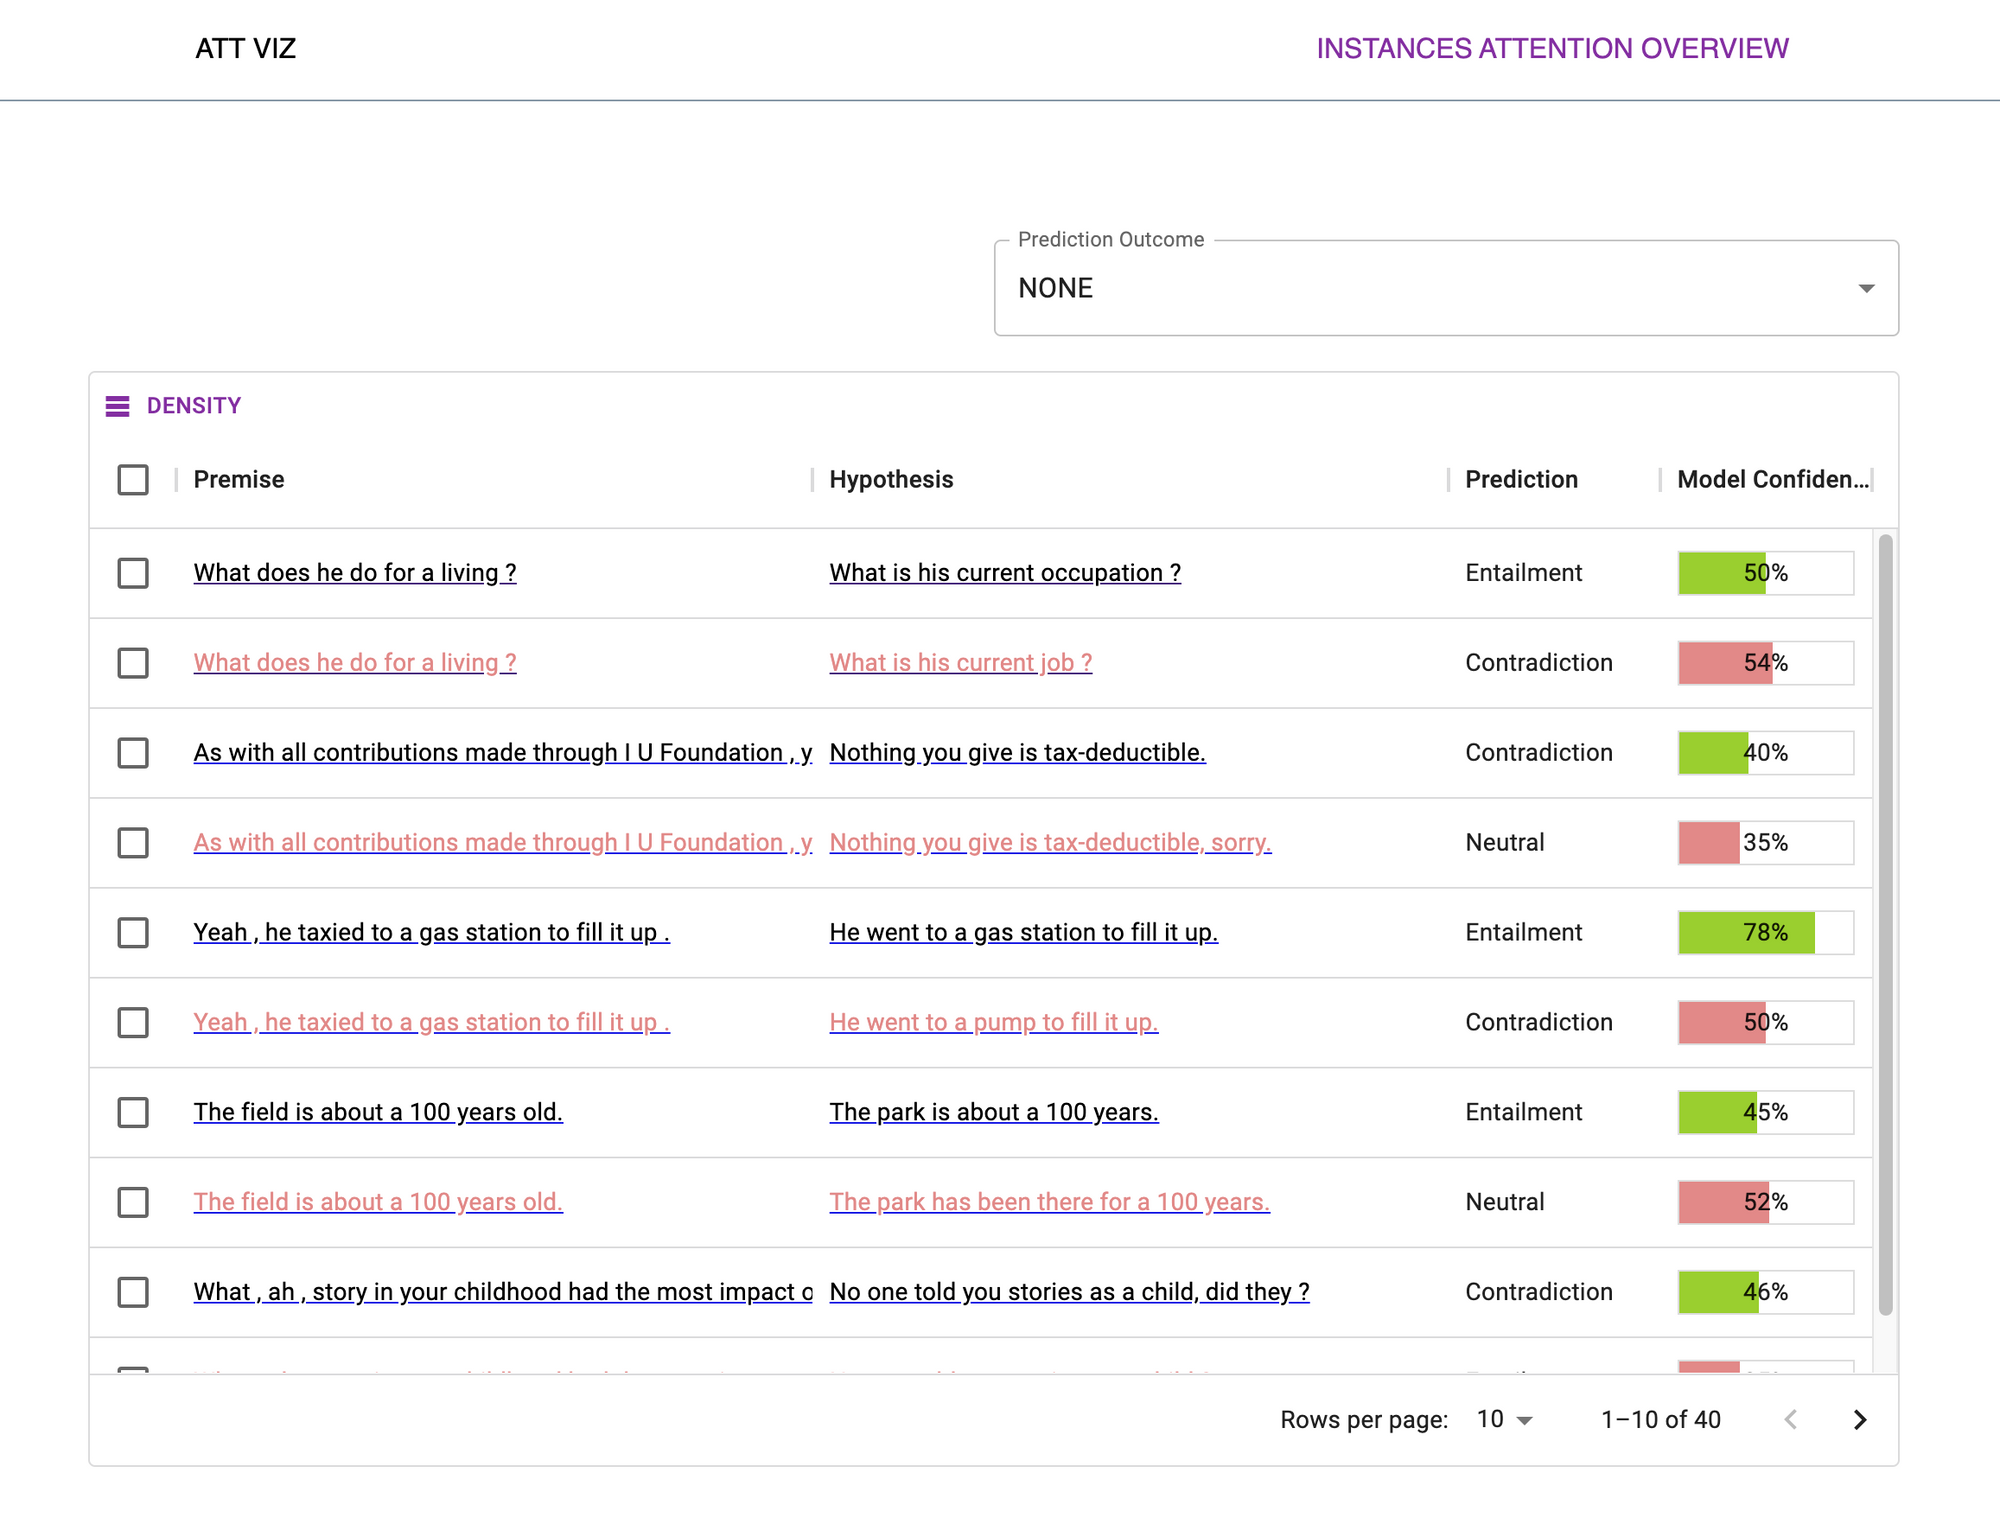
\includegraphics[width=8cm]{figures/Instance_Selection_View.png}
    \caption{Instance Selection View. Samples in red are adversarial}
    \label{fig:instance_selection_view_visualization}
    
\end{figure}

\subsubsection{Instance Selection view} The Instance selection view (Figure \ref{fig:instance_selection_view_visualization}) provides a table listing of all instances against the fine tuned model being evaluated. This view allows users to view the models confidence scores for the various data instances. Furthermore, the confidence scores are represented using horizontal bars where the size of the bar corresponds to the confidence level, meanwhile the colour of the bar represents whether the model predicted correctly for the provided instance. Users can sort the model’s columns by the confidence score, they are also able to view the models prediction for each instance in the data. Selecting the check boxes in the first column of the table will narrow down the instances shown to only the adversarial pair of the selected example. Users can also filter the table by the prediction outcome by selecting from a dropdown with options to see examples that passed or failed. 

Clicking on an instance navigates user to the Attention Head Overview view (Figure \ref{fig:attention_head_overview_visualization}) where users can view attention head details for each model in question.

\begin{figure}[h]
    \centering
    
    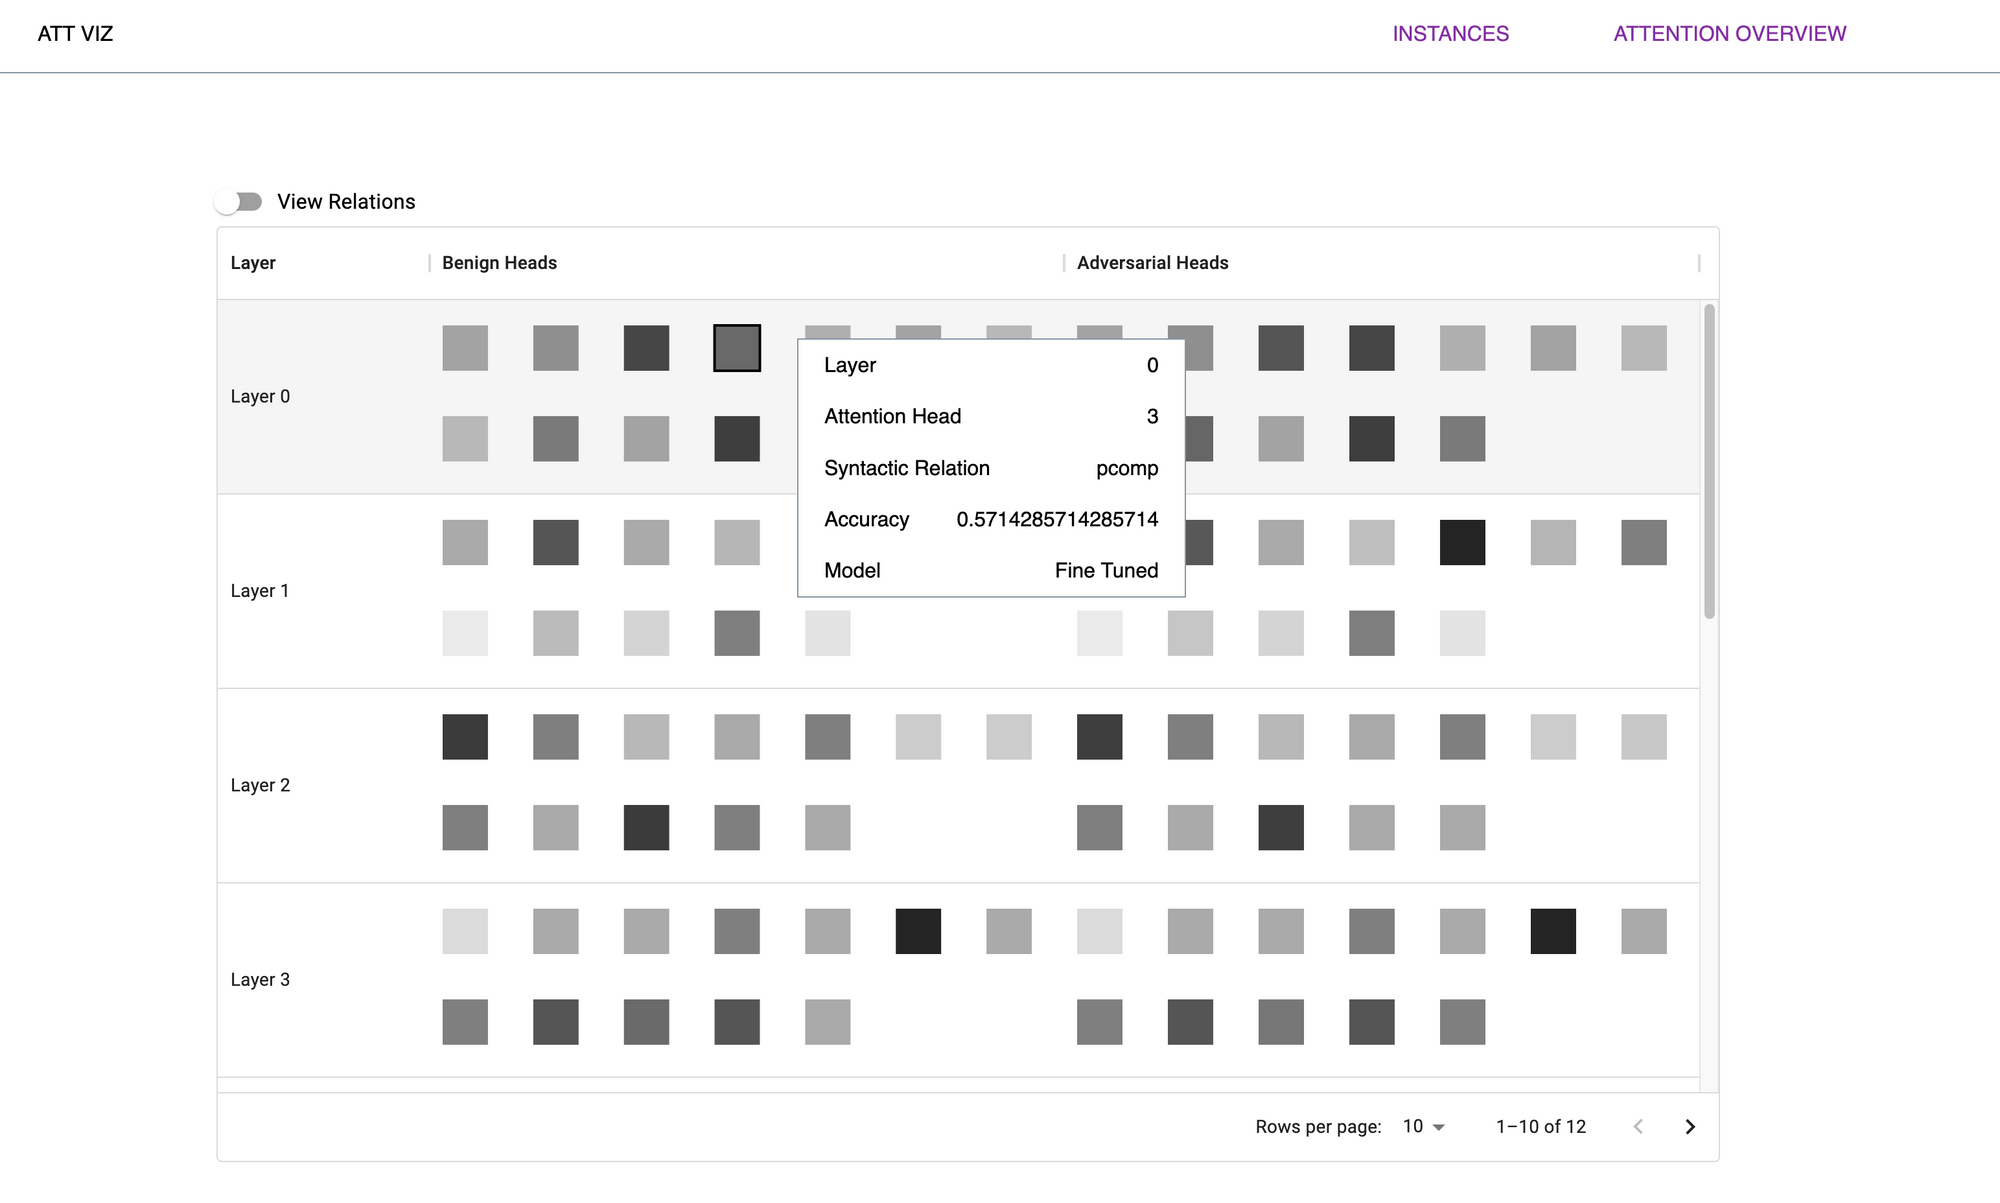
\includegraphics[width=8cm]{figures/Attention_Head_Overview.png}
    \caption{Attention Head Overview}
    \label{fig:attention_head_overview_visualization}
    
\end{figure}

\begin{figure}[tb]
    \centering
    
    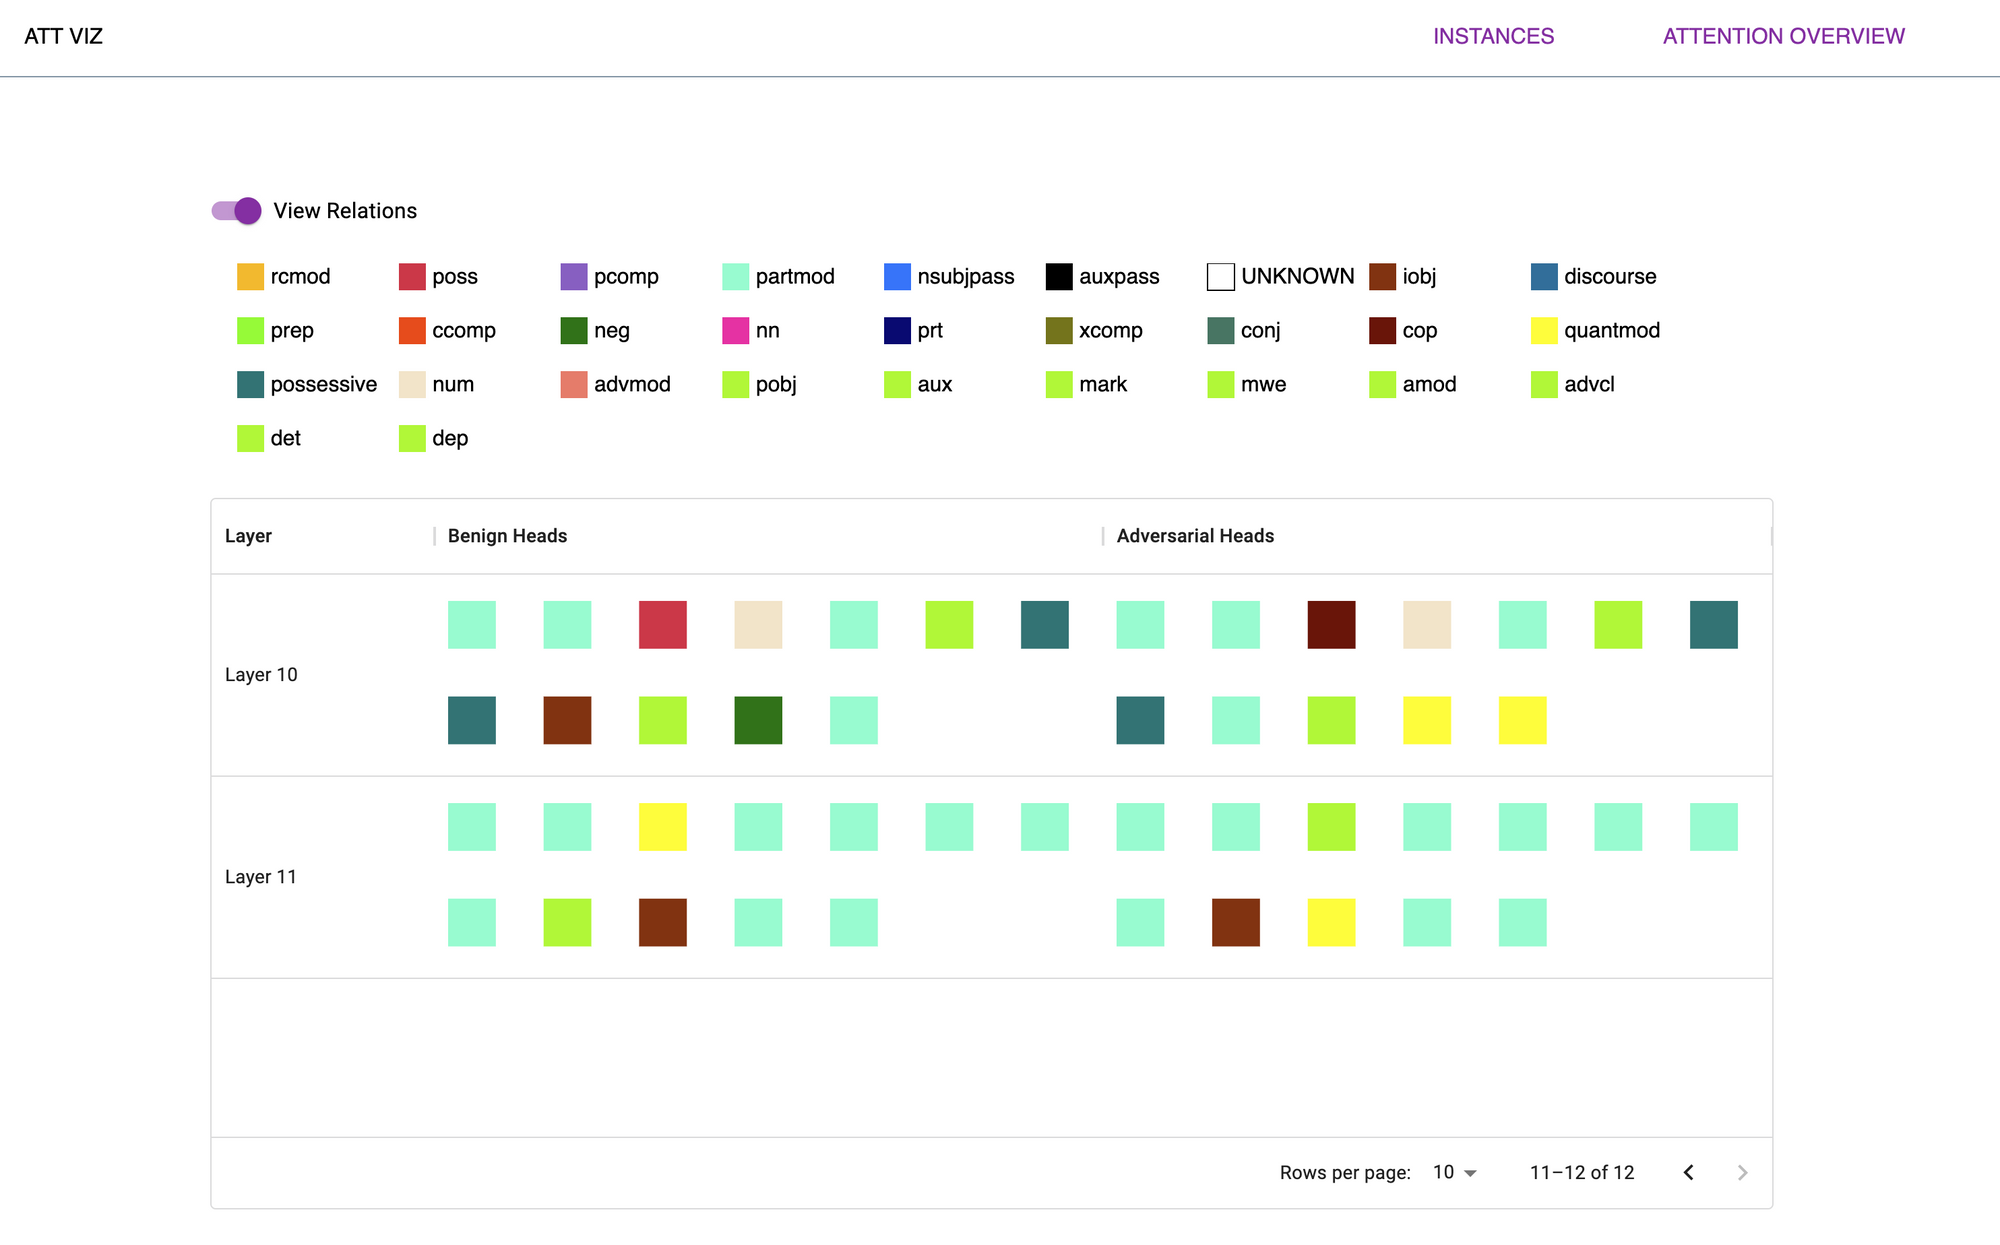
\includegraphics[width=8cm]{figures/Attention_Head_Overview_Syntactic.png}
    \caption{Attention Head Overview - Showing Syntactic Relations}
    \label{fig:attention_head_syntactic_visualization}
    
\end{figure}

\subsubsection{Attention Head Overview} This particular view provides a summary of of attention heads in each layer; and also provides a side by side comparison between attention heads of benign and adversarial examples. The view starts off by representing each attention head as black with various shades which represent how accurate the head extracts the syntactic relation in the provided sentence. Users are provided with the option to view the colored version of the overview. The colored version (as shown in Figure \ref{fig:attention_head_syntactic_visualization}) provides a clearer view of the various syntactic relations that each attention head focuses on. The various colors represent the aspect of the language that the attention heads have learned. One quick observation from analyzing the results showed that the adversarial and benign example attention heads start to look similar as we go deeper down the layers. 

In addition to using colors and shades of the attention head squares, numerical information is also rendered on a tooltip which users can view on-hover over an attention head. Hovering over a specific attention head in a model shows a tooltip that contains information about that particular attention head in a model, the layer, Syntactic relations, and how well the attention head performs at identifying the syntactic relation.


\begin{figure}[!htb]
    \centering
    
    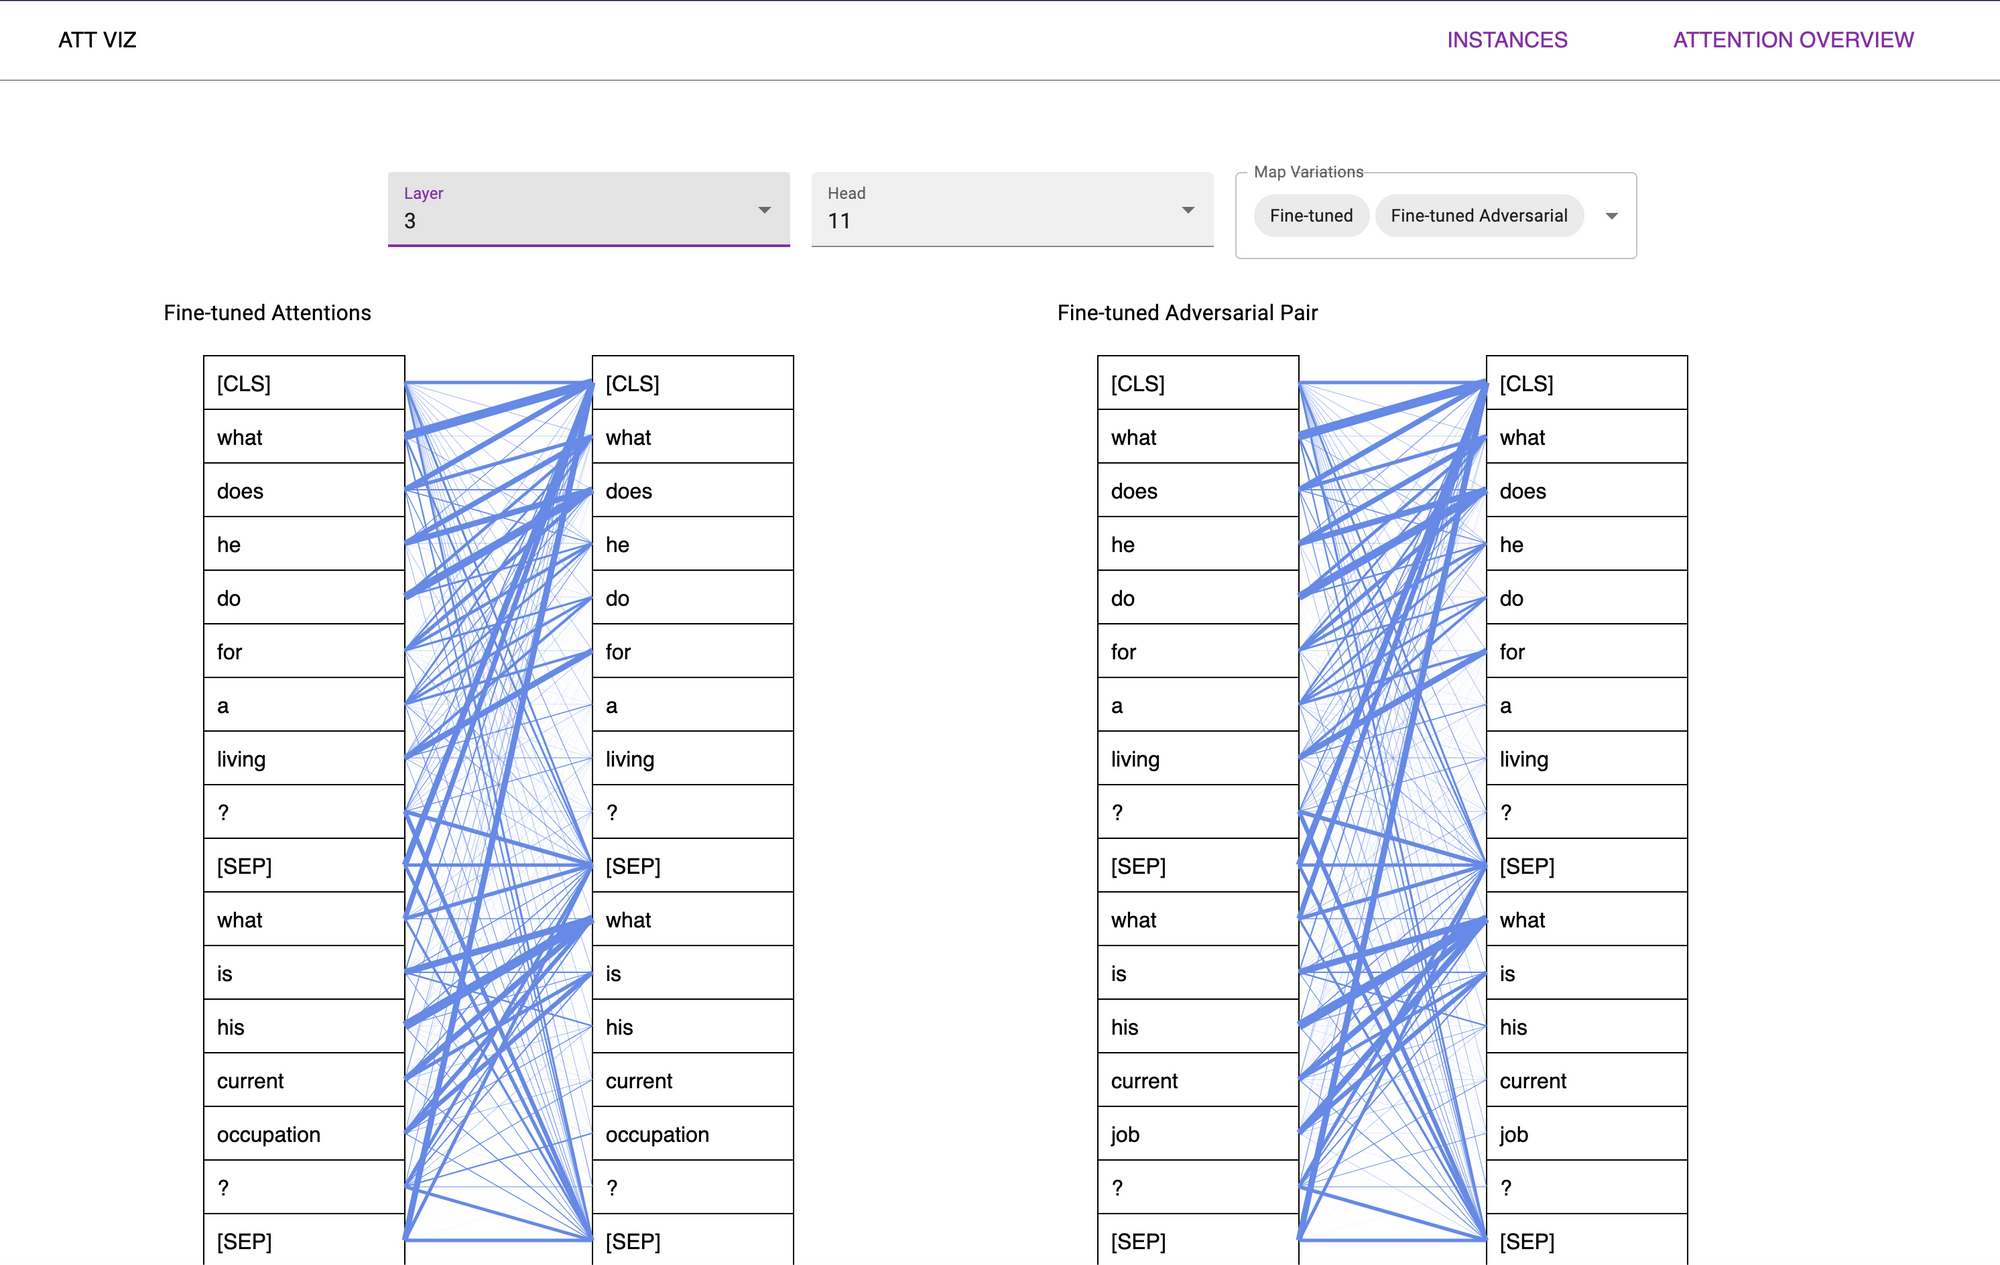
\includegraphics[width=8cm]{figures/Attention_Head_Instance_View.png}
    \caption{Attention Head Instance View}
    \label{fig:attention_head_instance_view_visualization}
    
    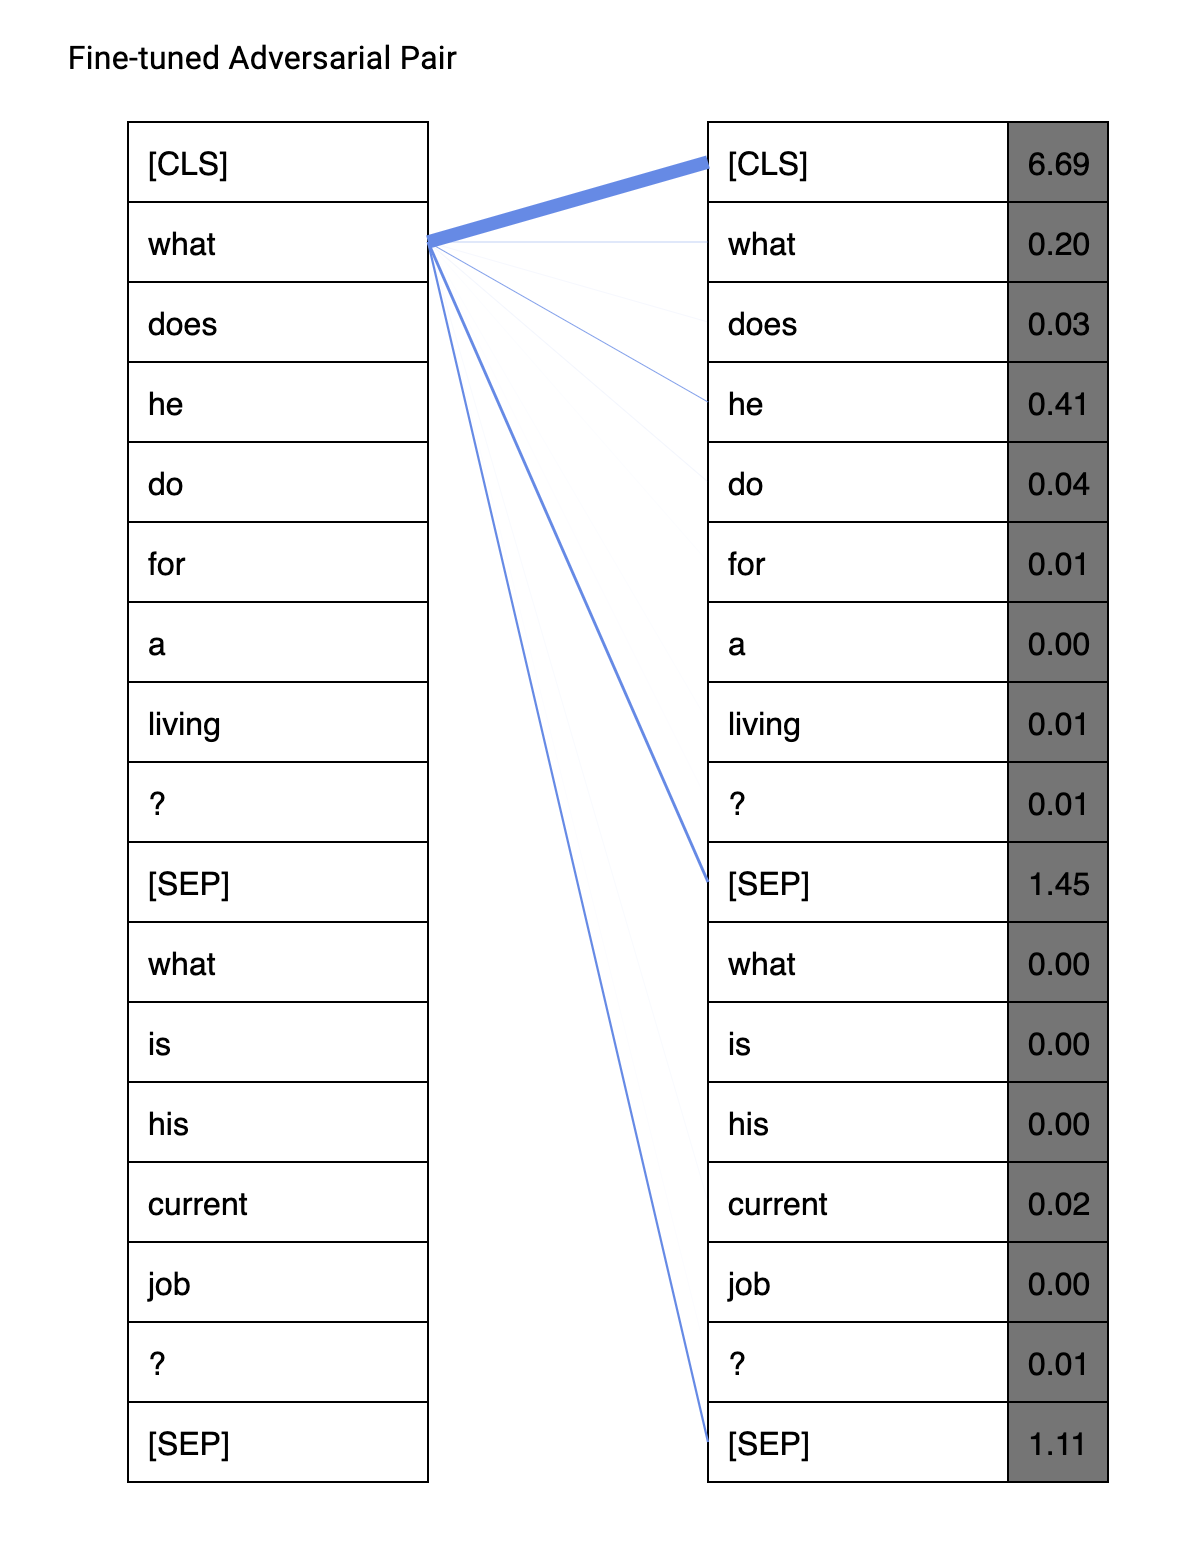
\includegraphics[width=8cm]{figures/Attention_Head_Instance_View_interaction_2.png}
    \caption{Attention Head Instance View Interaction}
    \label{fig:attention_head_instance_view_interaction_visualization}
    
\end{figure}

\subsubsection{Attention Head Instance View}
When a user clicks on a specific attention head, they are led to another view where they are presented with the attention map for the selected instance. In this view, the users can drill down to view the attention scores for each tokens in the instance. The user can also verify whether or not the detected syntactic relation identified is correct from this view. 

Within this view, users can adjust the layer they want to analyze, the attention head number, the model as well as the adversarial examples map for the selected instance. The number of attention maps a user can visualize at once is limited to 2 to try reducing clutter. 

Figure \ref{fig:attention_head_instance_view_interaction_visualization} - When a user hovers over a token, they are presented with the attention scores for that token. The number of displayed links are also filtered down to only show links for the token being inspected. We also highlight the token with the max score to make it easier for the user to identify them.
 



Our aim is that our visualizations can help model designers identify the cause of vulnerability to adversarial examples and provide actionable insights which can help them improve their training algorithms. Our improvements over existing transformer visualization include a view showing multiple instances and their confidence scores, ability to compare models and a less cluttered interface. 

% Transformer models dominate natural learning processing (NLP) leaderboards for many important applications such as Natural Language Inference (NLI), machine translation, speech recognition etc. Since these are black box methods researchers have turned to visualization techniques to help understand the representations that these models learn. Some methods focus on a specific aspects of the transformer architecture such as relation between attention and outputs~\cite{jain2019attention}, analysis of multi-headed attention~\cite{voita2019analyzing}, analysis of learned linguistic concepts~\cite{tenney2019bert} and role of intermediate layers~\cite{song2020utilizing}. Other methods~\cite{vig-2019-multiscale, aken2020visbert, vskrlj2020attviz, kobayashi-etal-2020-attention} look at the entire transformer architecture holistically and visualize embeddings, position heads, attention maps and even corpora.

% In this project we will consider two important NLP applications NLI and paraphrase detection. We will first train the transformer model on the  training sets, MNLI~\cite{williams-etal-2018-broad} and QQP~\cite{wang2017bilateral} respectively, and then analyze model performance on the `regular' evaluation set and the adversarial evaluations sets. HANS~\cite{mccoy2019right} is an adversarial dataset which has been designed for MNLI and PAWS~\cite{yang-etal-2019-paws} has been designed for QQP. We will integrate a holistic transformer visualization technique such as BertViz~\cite{vig-2019-multiscale}. BertViz is an interactive tool for visualizing embeddings and attention in Transformer language models such as BERT, GPT2, or T5. With a few upgrades to the BertViz visualizations we will explore whether these visualizations can help us diagnose model failure under the influence of adversarial examples and help us propose methods to mitigate it and design robust and reliable deep learning based NLP applications. An example of an upgrade to BertViz would be to represent vectors on a 2D plane as opposed to having an array of colors as it is much easier to use length to encode the relationship between vectors.

\section{Use Case}

We gave our application to Alan (fictional name) who works at a large technology company which deploys PLMs for a number of different products. They frequently face the issue that models when deployed \textit{in the wild} have significantly lower accuracy than when evaluated on clean data in-house. Alan sometimes uses adversarial examples as a proxy to test general robustness of the model. 

Alan takes our model and initially likes that unlike prior work he can look at multiple examples and select ones where the model makes a mistake on the adversarial example. He selects an adversarial example which leads the model to make a mistake. He selects the same example that we have introduced in Figure~\ref{fig:textfooler}. Next he looks at the Attention Head Overview and is curious about the different shades and the colors that he sees. He knows that the colors represent the syntactical relationships and the greyscale shades the accuracy of a particular attention head. Based on knowledge of these models Alan thinks that an attention head which can act as a participle modifier can give him some insight. On layer 11 (Figure~\ref{fig:partmod}) we can observe that attention head 10 is a participle modifier for both the benign and adversarial example. He selects this attention head to further analyze the attention scores.

\begin{figure}[h]
    \centering
    
    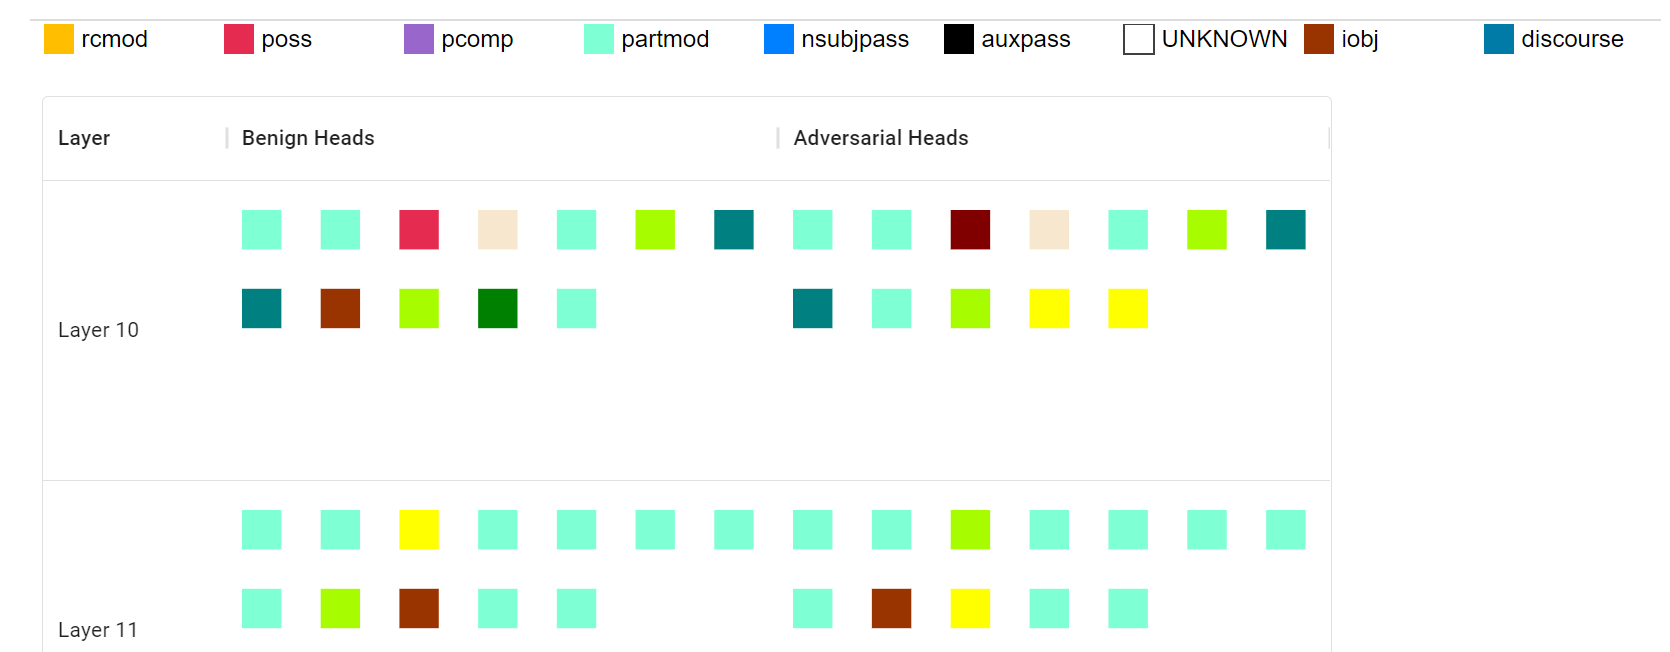
\includegraphics[width=8cm]{figures/partmod.png}
    \caption{Filtering attention head based on one that detects a partmod (participle modifier) relationship for both benign and adversarial sentence.}
    \label{fig:partmod}
    
\end{figure}

When he observes the attention (Figure~\ref{fig:usecase}) and hovers over the word that is changed (job to occupation) he observes that the attention score to the premise word living (synonym of job and occupation for this example) is lower in the adversarial example. On the other hand it has a stronger attention to the sentence separator. Alan observes that this is a recurring pattern and the model overfits to particular words. One remedy is to use data augmentation where the augmented data has synonyms of the nouns and verbs in the sentence.


\begin{figure}[h]
    \centering
    
    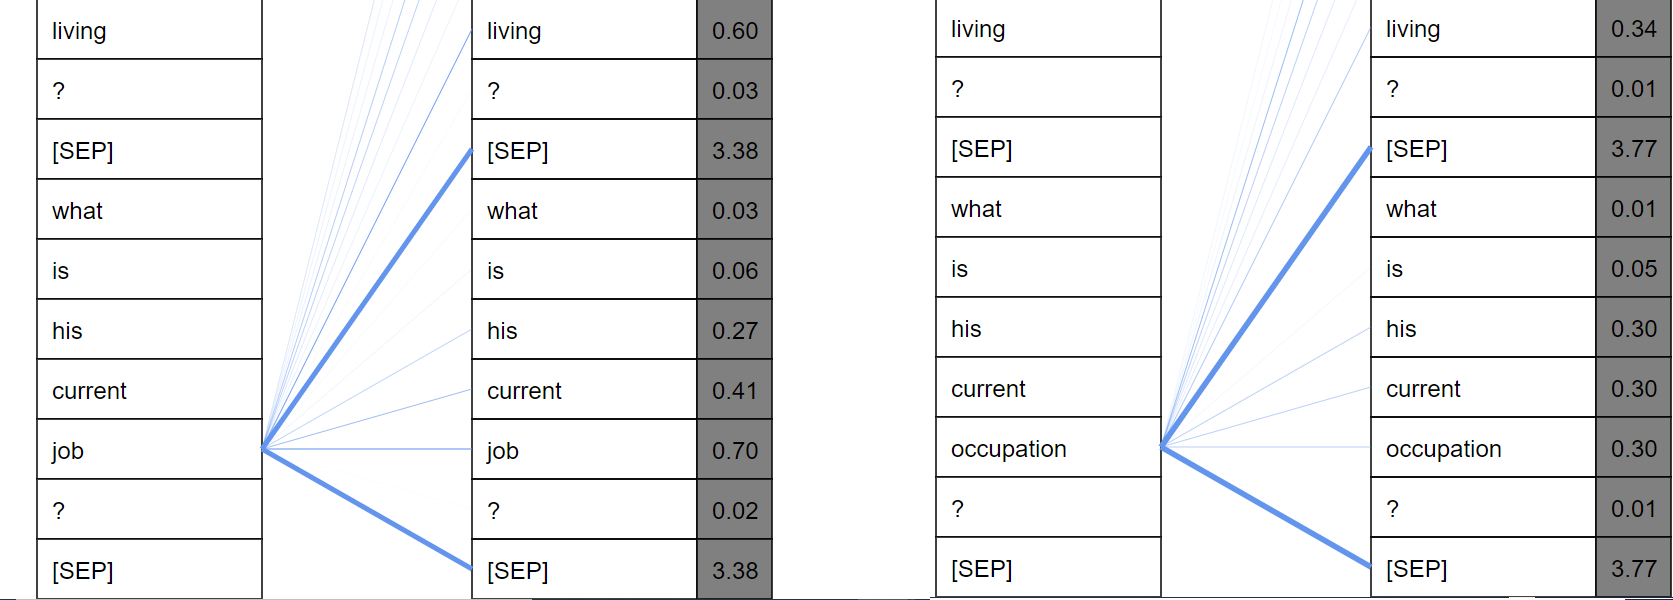
\includegraphics[width=8cm]{figures/usecase.png}
    \caption{Analyzing the difference in attention patterns between benign and adversarial example}
    \label{fig:usecase}
    
\end{figure}


Another interesting observation that Alan has is when comparing pre-trained and fine-tuned models even though only some of the parameters change, the attention patterns are completely re-arranged.

\section{Discussion}
The main contribution of our work is it helps domain experts such as linguists understand what transformers learn and help ML researchers gain insights of how to make the NLP model more robust. Users can compare models with different level of fine tuning and choose an appropriate level of fine tuning (whose internals appear to be more robust to adversarial examples). We provide the ability to compare different transformer models and also models based on benign and adversarial examples.

Although filtering based on syntactic patterns is useful in preliminary experiments, syntactic information is distributed over different attention heads. This information is helpful for linguists or NLP experts but to users from a different domain it is still difficult to understand where to look at. The tool itself is modular and can integrate other information such as semantic properties to filter attention heads. However going over the literature syntax looked the best option. One possible workaround is to filter out all the attention heads which achieve lower accuracy than a predefined threshold (such as 80\%). This is left for future work.

Another challenge in this work is although looking at attention patterns can lead to some understanding of why an NLP model behaves in a certain way, it is difficult to convert it into modeling insight. Our user Alan could come up with a training strategy because in this case we could see changes due to a synonym. But in other adversarial examples it might not be straightforward to come up with an idea to modify training. 



\section{Future Work}
One of the problems we noticed is that self-attention scores matrix is huge for any practical NLP model, and its size grows exponentially with the length of sentences as well. Since we need to generate, save and load these attention matrices, we have limited the number of data instances to be displayed. In the future, we can explore database technologies to make it possible to store massive amount of structured data and also to make querying it more efficient.

Another problem is that we used a trained syntactic parser as ground truth labels in our Attention Head Overview, but the prediction outputs of this model can be inaccurate. Although it would be more accurate to use human annotators to manually label the input data, our approach requires less work from the users as they do not have to supply labeled dataset. However, in the future we can add an option which allows users to supply their own labels which they deem more accurate. We can let users download our predicted labels and use it as a starting point.

It is difficult to compare different sized models as there is no one-to-one attention head interpretation. Our work currently requires the base transformers for the models under comparison to have the same structure. In the future we can explore ways to lift this requirement and allows meaningful comparisons of models based on transformers of different sizes.

The information learned by attention heads is usually distributed over multiple attention heads. Thus, looking at each attention head by itself is perhaps not ideal. In the future we can explore intelligent ways of automatically aggregating attention heads and let users customize the aggregation as well.


\acknowledgments

% Literature Review: Ahmad Rashid contributed to Section 2.1 and 2.2 and merging the sections. Siqing Huo contributed to section 2.2 and 2.3. Temiloluwa P. Femi-Gege and Shaikh S. A. Shimon contributed to Section 2.4. All authors help review the final submission. 

% Proposed Designed: Ahmad Rashid contributed to Section 3.1 and review and edit. Temiloluwa P. Femi-Gege contributed to Section 3.2 and 3.3. Shaikh S. A. Shimon contributed to Section 3.3. Siqing Huo worked on general editing and review and is working on code for the next submission.

\begin{itemize}
    \item Ahmad Rashid: Machine Learning code and writeup, use cases, discussion and integration
    \item Siqing Huo: Machine Learning Code and writeup, future works, integration and final editing.
    \item Temiloluwa P. Femi-Gege: Visualization design, code and writeup
    \item Shaikh S. A. Shimon: Abstract, Introduction and literature review
    
\end{itemize}





%\bibliographystyle{abbrv}
\bibliographystyle{abbrv-doi}
%\bibliographystyle{abbrv-doi-narrow}
%\bibliographystyle{abbrv-doi-hyperref}
%\bibliographystyle{abbrv-doi-hyperref-narrow}

\bibliography{template}
\end{document}

